\documentclass[aspectratio=169]{beamer}

\setbeamersize{text margin left=5mm, text margin right=5mm}

\defbeamertemplate{headline}{my header}{%
\vskip1pt%
\makebox[0pt][l]{\,\insertshortauthor}%
\hspace*{\fill}\insertshorttitle/\insertshortsubtitle\hspace*{\fill}%
\llap{\insertpagenumber/\insertpresentationendpage\,}
}
\setbeamertemplate{headline}[my header]

\let\olditem\item
\renewcommand{\item}{\setlength{\itemsep}{\fill}\olditem}

\usepackage{bm}
\usepackage{graphicx}
\usepackage{caption}
\usepackage{soul}
\usepackage{tkz-euclide}
\usetikzlibrary{calc}
\usepackage[]{algorithm2e}
\usepackage{changepage}
\usepackage{amssymb}
\usepackage{xcolor}
\usepackage{mathtools}
\usepackage{tcolorbox}
\usepackage{tikz}
\usepackage{tikz-3dplot}
\usepackage{tkz-euclide}
\usepackage{circuitikz}
\usepackage{mleftright}
\usetikzlibrary{arrows.meta, decorations.pathreplacing, positioning, shapes.geometric}
\usetikzlibrary{arrows}

\usepackage{pgfplots}
\usetikzlibrary{plotmarks}
\pgfplotsset{width=7cm,compat=1.8}
\pgfplotsset{compat=1.17}

\usetikzlibrary{positioning}
% \usepackage[math]{cellspace}
% \cellspacetoplimit 4pt
% \cellspacebottomlimit 4pt
%\usetikzlibrary{arrows.meta}
% sqare of half axes
\newcommand{\asa}{3}
\newcommand{\bsa}{1}
\newcommand{\csa}{0.25}
% view angle
\tdplotsetmaincoords{70}{135}


%% Fonts
\usefonttheme{professionalfonts}
\usefonttheme{serif}

\DeclareCaptionLabelFormat{blank}{}
\captionsetup[figure]{labelformat=blank}

%% Math definitions
\def\mf{\ensuremath\mathbf}
\def\mb{\ensuremath\mathbb}
\def\mc{\ensuremath\mathcal}
\def\lp{\ensuremath\left(}
\def\rp{\ensuremath\right)}
\def\lv{\ensuremath\left\lvert}
\def\rv{\ensuremath\right\rvert}
\def\lV{\ensuremath\left\lVert}
\def\rV{\ensuremath\right\rVert}
\def\lc{\ensuremath\left\{}
\def\rc{\ensuremath\right\}}
\def\ls{\ensuremath\left[}
\def\rs{\ensuremath\right]}
\def\bmx{\ensuremath\begin{bmatrix*}[r]}
\def\emx{\ensuremath\end{bmatrix*}}
\def\bmxc{\ensuremath\begin{bmatrix*}[c]}
\def\t{\lp t\rp}
\def\k{\ls k\rs}

\newcommand{\demoex}[2]{\onslide<#1->\begin{color}{black!60} #2 \end{color}}
\newcommand{\demoexc}[3]{\onslide<#1->\begin{color}{#2} #3 \end{color}}
\newcommand{\anim}[3]{\onslide<#1->{\begin{color}{#2!60} #3 \end{color}}}
\newcommand{\ct}[1]{\lp #1\rp}
\newcommand{\dt}[1]{\ls #1\rs}
\newcommand{\cols}[2]{\begin{columns}[#1] #2 \end{columns}}
\newcommand{\col}[2]{\begin{column}{#1} #2 \end{column}}

%% Mycolors
\definecolor{myred}{RGB}{192,0,0}
\definecolor{mygray}{RGB}{100,100,100}

%% Custom beamer color
\setbeamercolor{title}{fg=myred}
\setbeamercolor{subtitle}{fg=myred}
\setbeamerfont{title}{series=\bfseries}
% \setbeamercolor{frametitle}{bg=myred, fg=white}
\setbeamercolor{frametitle}{bg=mygray!10!, fg=myred}
\setbeamerfont{frametitle}{series=\bfseries}
\setbeamercolor{item}{fg=mygray}
\setbeamercolor{title in head/foot}{fg=myred}

% Move header to footer
\setbeamertemplate{headline}{}
\setbeamertemplate{footline}{
  \begin{beamercolorbox}[wd=\paperwidth,ht=2.25ex,dp=1ex,center]{footline}
    \inserttitle\hfill\insertauthor\hfill\insertdate\hfill\insertframenumber{}
  \end{beamercolorbox}
}

\pgfplotsset{
colormap={whitered}{color(0cm)=(white); color(1cm)=(orange!75!red)}
}


\title{Applied Linear Algebra for Data}

% A subtitle is optional and this may be deleted
\subtitle{Probability and Statistics}

\author{Sivakumar Balasubramanian}
% - Give the names in the same order as the appear in the paper.
% - Use the \inst{?} command only if the authors have different
%   affiliation.

\institute[Christian Medical College] % (optional, but mostly needed)
{
  \inst{}%
  Department of Bioengineering\\
  Christian Medical College, Bagayam\\
  Vellore 632002
}
% - Use the \inst command only if there are several affiliations.
% - Keep it simple, no one is interested in your street address.

\date{}
% - Either use conference name or its abbreviation.
% - Not really informative to the audience, more for people (including
%   yourself) who are reading the slides online

\subject{Lecture notes on ALADA}
% This is only inserted into the PDF information catalog. Can be left
% out. 

% If you have a file called "university-logo-filename.xxx", where xxx
% is a graphic format that can be processed by latex or pdflatex,
% resp., then you can add a logo as follows:

% \pgfdeclareimage[height=0.5cm]{university-logo}{university-logo-filename}
% \logo{\pgfuseimage{university-logo}}

% Delete this, if you do not want the table of contents to pop up at
% the beginning of each subsection:
\AtBeginSubsection[]
{
  \begin{frame}<beamer>{Outline}
    \tableofcontents[currentsection,currentsubsection]
  \end{frame}
}

% Let's get started
\begin{document}

\pgfplotsset{
  compat=1.8,
  colormap={whitered}{color(0cm)=(white); color(1cm)=(orange!75!red)}
}


\begin{frame}
  \titlepage
\end{frame}

% \begin{frame}[t]{References}
% \begin{itemize}
%     \item G Strang, Linear Algebra: Chapters .
% \end{itemize} 
% \end{frame}


\begin{frame}[t]{Probability and Statistics}
\begin{itemize}
    \item Uncertainity is ubiquitous in everything that we do.
    
    \item Probability is a mathematical framework to model uncertainity.  

    \item Statistics is a branch of mathematics that is about collecting, analyzing, interpreting, and presenting data.
    
    \item Probability theory forms the foundation of statistics.
    
    \item This lecture will provide a very brief introduction to probability and statistics, focusing on some of the most important concepts.
\end{itemize}
\end{frame}


\begin{frame}[t]{Probability theory: a brief review}
\begin{itemize}
    \item What is probability? Consider the statement: \textit{The probability of coin landing heads is 0.75.} What does this mean?
    
    \item Two views: \textbf{Frequentist} and \textbf{Bayesian}.
    
    \item \textbf{Frequentist view}: Probability is the long run relative frequency of an event. If we 
    toss a coin $N=1000$ times, we expect it to land heads around $n_H = 700$ times.
    \[ p = \lim_{N\to\infty} \frac{n_H}{N} = 0.75 \]
    
    \item \textbf{Bayesian view}: Probability is a measure that quantifies our uncertainity about an event. This view associates probability with information about something and not repeated trials. For example, here we believe that the coin is three times more likely to turn uop heads than tails when the probability is 0.75.
    
    \item Beyond these philosophical differences, both approaches can lead to differences in results in practice.
\end{itemize}
\end{frame}


\begin{frame}[t]{Fundamental rules of probability}
\begin{itemize}
  \item \textbf{Random experiment} -- A experiment whose outcome is not predictable.
  
  \begin{itemize}
    \item Tossing of a coin.
    \item Voltage across a real resistor $\ct{R}$ for a known current.
    \item Height and weight of 40 year old person randomly chosen from a population.
  \end{itemize}

  \item The \textbf{outcome} of a random experiment is any observable variable of interest.

  \item \textbf{Sample space} of the experiment $S$ is the universe of possible values we can observe for a random experiment's outcome.

  \item An \textbf{event} of an experiment is any subset of the sample space $S$.
\end{itemize}
\end{frame}


\begin{frame}[t]{Fundamental rules of probability}
\begin{itemize}
  \item Consider the experiment tossing a dice, and we observe the count of the dots that turn on the top face of the dice.
  \begin{itemize}
    \item Observed outcome is an even number. $A = \lc 2, 4, 6\rc \subset S$
    \item Observed outcome is a positive number. $A = S \implies $ \textbf{Sure event}
    \item Observed outcome is 0. $A = \lc\rc \implies $ \textbf{Impossible event}
  \end{itemize}
  
  \item For discrete sample spaces and \textbf{elementary event} is an event with just single sample point.
  
  \item We can combine events to produce other events that might be of interest to us. Set operations can be used to perform algebra on events.
\end{itemize}
\end{frame}


\begin{frame}[t]{Fundamental rules of probability}
\begin{itemize}
  \item Let $A$ be an event of an experiments, and $p\ct{A}$ the probability of the event $A$.
  
  \item The assignment of probabilities satisfies the following prorperties.
  \begin{itemize}
    \item For any event $A$, $0 \leq P\lp A \rp \leq 1$.
    \item $P\lp S \rp = 1$; $S$ is the sample space.
    \item For two events $A, B$, 
    \[ \begin{cases}
      A \cap B = \emptyset & \implies P\lp A \cup B\rp = P\lp A\rp + P\lp B\rp\\
      A \cap B \neq \emptyset & \implies P\lp A \cup B\rp = P\lp A\rp + P\lp B\rp - P\lp A \cap B\rp
       \end{cases} \]
  \end{itemize}

  \item  The other rules for proability calculation for events of an experiment can be derived from these three axioms.
  \begin{itemize}
    \item $P\lp \overline{A}\rp = 1 - P\lp A \rp$
    \item $A \subset B \, \implies P\lp A \rp \leq P\lp B\rp$
    \item $P\lp \emptyset \rp = 0$
    \item $P\lp A \cup B \rp = P\lp A\rp + P\lp B\rp - P\lp A \cap B\rp$
  \end{itemize}
\end{itemize}
\end{frame}


\begin{frame}[t]{Random variables}
\begin{itemize}
  \item A random variable is $X$ is a function that maps the sample space $S$ to the real numbers $\mb{R}$. Random variables allow us to deal with experimental outcomes and event interms of numbers instead of arbitrary symbols. Note: We will use ``r.v.'' to mean ``random variable'' from this point on.
  
  \item Two types of random variables: Discrete random variables and Continuous random variables.
  
  \item Discrete random variables take on values from a discrete set of numbers $\mathcal{X}$ (finite or countably infinite).
  
  \item Continuous random variables take on values from a continuous set of numbers $\mathcal{X}$ (uncountably infinite).
  
  \item Function that assigns probabilities to a discrete random variable $X$ is called the \textbf{proability mass function} (p.m.f.) $p\ct{X = x}$ is the proability of the random variable $X$ assuming the value $x$.
  \[ p\ct{X = x} \geq 0, \,\,  \forall x \in \mc{X}, \quad \quad \sum_{\mc{X} \in x} p\ct{X = x} \geq 0 \]
\end{itemize}
\end{frame}


\begin{frame}[t]{Random variables}
  \vspace{-0.25cm}
  Here are two proability mass fucntions.
  \begin{center}
    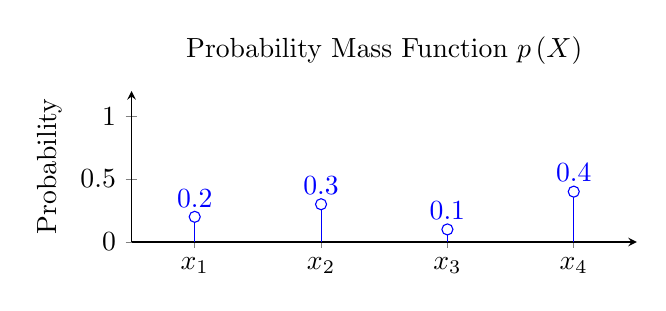
\begin{tikzpicture}
      \begin{axis}[
        ycomb, % Use ycomb style for stem plot
        width=8cm,
        height=3.5cm,
        ylabel={Probability},
        ymin=0,
        ymax=1.2,
        xmin=0.5, % Adjust the x-axis minimum value to shift it to the left
        xmax=4.5, % Adjust the x-axis maximum value to shift it to the left
        xtick={1, 2, 3, 4}, % Specify the numerical x-values
        xticklabels={$x_1$, $x_2$, $x_3$, $x_4$},
        nodes near coords,
        nodes near coords align={vertical},
        axis lines=left, % Specify only left and bottom axes lines
        title={Probability Mass Function $p\lp X \rp$}, % Add a title here
        ]
        
        % Define your data points and corresponding probabilities
        \addplot +[mark=*, mark options={fill=white}] coordinates {(1, 0.2) (2, 0.3) (3, 0.1) (4, 0.4)};
    \end{axis}
    \end{tikzpicture}

    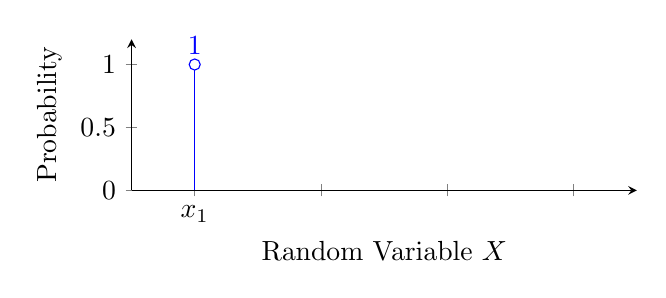
\begin{tikzpicture}
      \begin{axis}[
        ycomb, % Use ycomb style for stem plot
        width=8cm,
        height=3.5cm,
        xlabel={Random Variable $X$},
        ylabel={Probability},
        ymin=0,
        ymax=1.2,
        xmin=0.5, % Adjust the x-axis minimum value to shift it to the left
        xmax=4.5, % Adjust the x-axis maximum value to shift it to the left
        xtick={1, 2, 3, 4}, % Specify the numerical x-values
        xticklabels={$x_1$},
        nodes near coords,
        nodes near coords align={vertical},
        axis lines=left, % Specify only left and bottom axes lines
        ]
        
        % Define your data points and corresponding probabilities
        \addplot +[mark=*, mark options={fill=white}] coordinates {(1, 1.0) };
    \end{axis}
    \end{tikzpicture}
  \end{center}
\end{frame}


\begin{frame}{Joint and Marginal Probabilities}
  \begin{itemize}
    \item Consider two r.v. $X \in \mc{X}$ and $Y \in \mc{Y}$. The joint p.m.f. of these r.v. is defined as,
    \[ p\lp X = x, Y = y\rp = p\lp \lc X = x\rc \cap \lc Y = y \rc \rp = p\lp Y = y, X = x\rp \]
    \textbf{Meaning of joint probabilities}: $p\lp X = x, Y = y\rp$ is the probability of the r.v. $X$ takes on the value $x$ \textbf{and} the r.v. $Y$ takes on the value $y$.
    
    \item The marginal p.m.f. of the r.v. $X$ is the probability that it takes on a value $x$. This can be computed from the joint p.m.f. as the following,
    \[ p\lp X = x \rp = \sum_{y \in \mc{Y}} p\lp X=  x, Y = y \rp \]
    Similary the margnal p.m.f. of r.v. $Y$ is
    \[ p\lp Y = x \rp = \sum_{x \in \mc{X}} p\lp X =  x, Y = y \rp \]
  \end{itemize}
\end{frame}


\begin{frame}{Conditional probabilities}
  \begin{itemize}
    \item Consider two r.v. $X \in \mc{X}$ and $Y \in \mc{Y}$, with the joint p.m.f. $p\lp X, Y\rp$.
    
    \item The conditional p.m.f $X = x$ given $Y = y$ is defined as,
    \[ p\lp X = x \vert Y = y \rp =  \frac{p\lp X = x, Y = y\rp}{p\lp Y = y \rp}, \,\, \mathrm{if } \,\, p\lp Y = y \rp \neq 0 \]
    The conditional proability is not defined if $p\lp Y = y \rp = 0$.

    \textbf{Meaning of conditional probabilities}: $p\lp X = x \vert Y = y \rp$ is the probability that r.v. $X$ taking on a value $x \in \mc{X}$, given that \textbf{we know} the r.v. $Y$ has taken on a value $y \in \mc{Y}$. 
    
    Note that $p\lp Y = y \rp = 0$ means that $Y = y$ cannot have occured, so there is nothing to condition on (i.e., the statement ``$Y$ has taken on a value $y \in \mc{Y}$'' is meaningless).
  \end{itemize}
\end{frame}


\begin{frame}{Bayes Rule}
  Consider two discrete r.v. $X$ and $Y$. We know the following conditional probabilities,
  \[ p\lp X \vert Y \rp =  \frac{p\lp X, Y\rp}{p\lp Y \rp} \quad \quad p\lp Y \vert X \rp =  \frac{p\lp X, Y\rp}{p\lp X \rp} \]
  (Note: we drop writing $X=x$ and $Y=y$ for brevity).

  Thus, we have the \textbf{Bayes rule} or \textbf{Bayes theorem},
  \[ \begin{split}
    p\lp X \vert Y \rp &= \frac{p\lp Y \vert X \rp p\lp X\rp}{p\lp Y \rp} = \frac{p\lp Y \vert X \rp p\lp X\rp}{\sum_{x \in \mc{X}} p\lp X = x, Y = y\rp}\\
                       &= \frac{p\lp Y \vert X \rp p\lp X\rp}{\sum_{x \in \mc{X}} p\lp Y \vert X = x\rp p\lp X = x \rp}  \\
  \end{split} \]
\end{frame}


\begin{frame}{Example of applying Bayes rule}
  \begin{columns}
    \begin{column}{0.7\textwidth}
      \vspace{0.25cm}
      
      \begin{small}
        You have written a python program that does some clever image processing to automatically detect pulmonary embolism (PB) using a given chest x-ray image. After extensive testing with data from CMC you've estblished that your program has a sensitvity of 85\%, i.e. your program will report that a person is +ve for PB from his/her chest x-ray image 85\% of the time when the person is indeed +ve for PB. And it has a specificity of 95\%, i.e. your program will report that a person is -ve for PB from his/her chest x-ray image 95\% of the time when the person is indeed -ve for PB. 
        \vspace{0.1cm}
        
        When I run your program on my most recent chest x-ray, your program reported that I am +ve for PB! Oh my god! Do I have PB? What is the probability that I have PB?
      \end{small}
    \end{column}
    \begin{column}{0.275\textwidth}
      \begin{figure}
        \centering
        
\includegraphics[width=0.8\textwidth]{figs/scared.png}
      \end{figure}
    \end{column}
  \end{columns}
\end{frame}


\begin{frame}{Independence}
  We say two r.v. $X$ and $Y$ are unconditionally independent or marginally independent, denoted by $X \perp Y$, if
  \[ X \perp Y \quad \iff \quad p\ct{X, Y} = p\ct{X}p\ct{Y} \]
    
  \textcolor{blue}{What does this mean?}
  \begin{itemize}
    \item The two r.v. do not carry any information about the other. \textcolor{gray}{Remember the $\perp$ symbol when talking about vectors. $\mf{x} \perp \mf{y} \implies$ $\mf{x}$ is perpendicular to $\mf{y}$. Informally, $\mf{x}$ does not carry any information about $y$ and \textit{vice versa}. The same idea applies here r.v. $X$ and $Y$. $X \perp Y \implies$ that r.v. $X$ contains no information about $Y$ and \textit{vice versa}.}
    \item The condition probability is the marginal probability, i.e. $p\ct{X \vert Y} = p\ct{X}$ and $p\ct{Y \vert X} = p\ct{Y}$.
    \item The p.m.f. of $X$ for any given values of $Y$ has the same shape as $p\ct{X}$, and similarly the p.m.f. of $Y$ for any given value of $X$ has the same shape as $p\ct{Y}$.
    \[ p\ct{X, Y=y} \propto p\ct{X} \quad \quad p\ct{X=x, Y} \propto p\ct{Y} \]
  \end{itemize}
\end{frame}


\begin{frame}{Conditional Independence}
  We say two r.v. $X$ and $Y$ are conditionally independent given a r.v. $Z$, denoted by $X \perp Y \vert Z$, if
  \[ X \perp Y \vert Z \quad \iff \quad p\ct{X, Y \vert Z} = p\ct{X \vert Z}p\ct{Y \vert Z} \]
    
  \textcolor{blue}{What does this mean?} $X$ carries not information about $Y$, and \textit{vice versa}, given that we know $Z$ took on some value $z$.
  \vspace{0.2cm}

  \textcolor{blue}{Theorem}:
  $X \perp Y \vert Z$ if and only if, there exist  functions $g$ and $h$ such that,
  \[ p\ct{X, Y \vert Z} = g\ct{X, Z} h\ct{Y, Z} \]
  for all $X, Y$ such that $p\ct{Z} > 0$.
\end{frame}


\begin{frame}{Continuous Random Variables}
  \begin{itemize}
    \item Let $X$ be a continuous r.v. such that $X \in \mc{X} \subseteq \mb{R}$.
    \item We can meaningfully define probabilities for continuous r.v. only for intervals of the real line. For example, we can define the probability that $X$ takes on a value in the interval $\ls a, b \rs \subset \mc{X}$.
    \item For a continuous r.v. $X$, we define a probability density function (p.d.f.) $f\ct{x}$ such that,
    \[ p\ct{a \leq X \leq b} = \int_{a}^{b} f\ct{X}dX \]
    Another useful function is the cummulative distribution function (c.d.f.) $F\ct{X}$, defined as,
    \[ p\ct{X \leq a} = F\ct{X} = \int_{-\infty}^{a} f\ct{X}dX \]
    \item For a small interval $\ls x, x + dx \rs$, the probability that $X$ takes on a value in this interval is $f\ct{X}dx$ $\longrightarrow f\ct{X} = \frac{p\ct{x, x+dx}}{dx}$.
  \end{itemize}
\end{frame}


\begin{frame}{Expected values of a random varaible}
  \textbf{Expected value of a r.v} is the average value of the r.v. over all possible outcomes. For a discrete r.v. $X$ with p.m.f. $p\ct{X}$, the expected value is,
  \[ \mb{E}\dt{X} = \sum_{x \in \mc{X}} x \cdot p\ct{X = x} \]
  For a continuous r.v. $X$ with p.d.f. $f\ct{X}$, the expected value is,
  \[ \mb{E}\dt{X} = \int_{\mc{X}} x \cdot f\ct{X = x} dX \quad \mathrm{or} \mb{E}\dt{X} = \sum_{x \in \mc{X}} x \cdot p\ct{X = x} \]
\end{frame}


\begin{frame}{Expected values of a random varaible}
  \textbf{Variance a r.v} is a measure of the spread of a r.v. about its mean.
  \[ \mathrm{var}\dt{X} = \mb{E}\dt{\ct{X - E\dt{X}}^2} = \mb{E}\dt{X^2} - \mb{E}\dt{X}^2 \]
  
  The square root of $\mathrm{var}\dt{X}$ is called the \textbf{standard deviation} of $X$.
  \[ \mathrm{std}\dt{X} = \sqrt{\mathrm{var}\dt{X} } \]

  We can compute the expected value of any function $g\ct{\bullet}$ of a r.v. $X$ as follows,
  \[ \mb{E}\dt{g\ct{X}} = \int_{\mc{X}} g\ct{X} \cdot f\ct{X} dX \]
\end{frame}


\begin{frame}{Covariance and Correlation between two r.v. $X$ and $Y$}
  Consider two r.v. $X$ and $Y$ with joint p.d.f. $f\ct{X, Y}$. The covariance between $X$ and $Y$ measures the (linear) relationship between the two r.v. This is defined as the following,
  \[ \mathrm{cov}\dt{X, Y} = \mb{E}\dt{\ct{X - \mb{E}\dt{X}}\ct{Y - \mb{E}\dt{Y}}} \]
  \vspace{0.05cm}
  
  $\mathrm{cov}\dt{X, Y}$ can take on any value between $-\infty$ and $\infty$. 
  \vspace{0.4cm}
  
  When $\mathrm{cov}\dt{X, Y}$ is normalized by the standard deviations of $X$ and $Y$, we get the correlation between $X$ and $Y$.
  \[ \mathrm{corr}\dt{X, y} = \frac{\mathrm{cov}\dt{X, Y}}{\sqrt{\mathrm{var}\dt{X}} \sqrt{\mathrm{var}\dt{Y}}} \] 
\end{frame}


\begin{frame}{Some discrete r.v. and their p.m.f.}
  \textbf{Bernoulli distribution} Used to model a single coin toss. The r.v. $X \in \lc 0, 1\rc$ takes on the value 1 if the coin lands heads, and 0 if the coin lands tails. The p.m.f. is,
  \[ p\ct{X = x; \theta} = \theta^X \cdot \ct{1 - \theta}^{\ct{1 - X}} \]
  where, $p$ is the probability of the coin turning up heads.
  \vspace{0.25cm}
  \begin{center}
    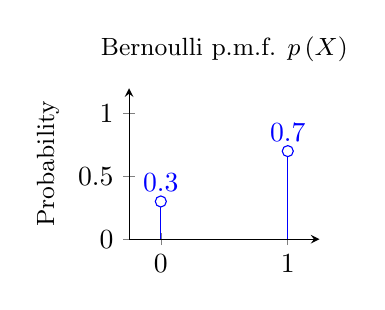
\begin{tikzpicture}
      \begin{axis}[
        ycomb, % Use ycomb style for stem plot
        width=4cm,
        height=3.5cm,
        ylabel={\small Probability},
        ymin=0,
        ymax=1.2,
        xmin=-0.25, % Adjust the x-axis minimum value to shift it to the left
        xmax=1.25, % Adjust the x-axis maximum value to shift it to the left
        xtick={0, 1}, % Specify the numerical x-values
        % xticklabels={$0$, $x_2$, $x_3$, $x_4$},
        nodes near coords,
        nodes near coords align={vertical},
        axis lines=left, % Specify only left and bottom axes lines
        title={\small Bernoulli p.m.f. $p\lp X \rp$}, % Add a title here
        ]
        
        % Define your data points and corresponding probabilities
        \addplot +[mark=*, mark options={fill=white}] coordinates {(0, 0.3) (1, 0.7)};
      \end{axis}
    \end{tikzpicture}
  \end{center}
\end{frame}


\begin{frame}{Some discrete r.v. and their p.m.f.}
  \textbf{Bionomial distribution} Used to model the result of experiment with $n$ independent coin tosses. The r.v. $X \in \lc 0, 1, \ldots, n\rc$ takes on the value $k$ if there are $k$ heads in $n$ tosses. The p.m.f. is,
  \[ p\ct{X = k; \theta, n} =  \frac{n!}{k! \ct{n - k}!} \cdot \theta^k \cdot \ct{1 - \theta}^{\ct{n - k}} \]
\end{frame}


\begin{frame}{Some discrete r.v. and their p.m.f.}
  \textbf{Poisson distribution} Used to model the number of events that occur in a fixed interval of time. The r.v. $X \in \lc 0, 1, \ldots\rc$ takes on the value $k$ if there are $k$ events in the interval. The p.m.f. is,
  \[ p\ct{X = k; \lambda} =  \frac{\lambda^k}{k!} e^{-\lambda} \]
  where, $\lambda$ is the average number of events in the interval.
\end{frame}


\begin{frame}{Some discrete r.v. and their p.m.f.}
  \textbf{Uniform distribution} Used to model the outcome of an experiment where all outcomes are equally likely. The r.v. $X \in \lc a, b\rc$ takes on the value $x$ with equal probability. The p.m.f. is,
  \[ \mathrm{Unif}\ct{X = x; a, b} =  \frac{1}{b - a} \mb{I}\ct{a \leq x \leq b} \]
  where, $\mb{I}\ct{A}$ is the indicator function, defined as the following
  \[ \mb{I}\ct{A} = \begin{cases}
    1 & \mathrm{if} \,\, A \,\, \mathrm{is} \,\, \mathrm{true}\\
    0 & \mathrm{if} \,\, A \,\, \mathrm{is} \,\, \mathrm{false} 
  \end{cases} \]
\end{frame}


\begin{frame}{Gaussian (Normal) distribution}
  \textbf{Gaussian Distribution} is the most commonly used statistical distribution, wose p.m.f. is defined as,
  \[ \mc{N}\ct{X=x; \mu, \sigma^2 } = \frac{1}{\sqrt{2\pi\sigma^2}} e^{-\frac{\ct{x - \mu}^2}{2\sigma^2}} \]
  where, $\mu$ is the mean of the distribution and $\sigma^2$ is the variance.
  \vspace{0.1cm}

  \begin{center}
    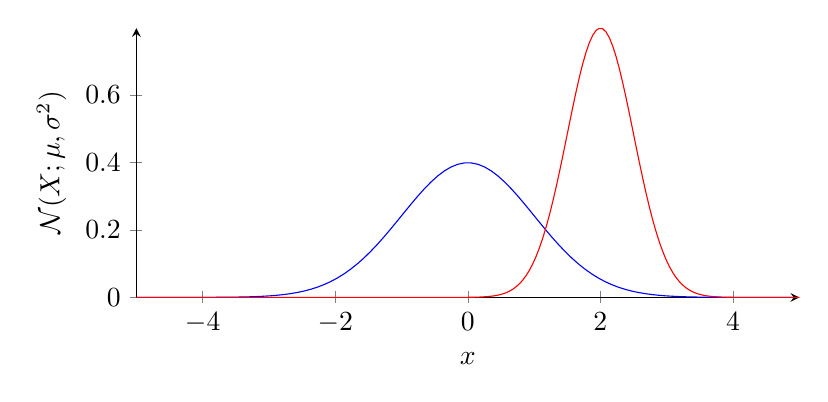
\begin{tikzpicture}
      \begin{axis}[
        width=10cm,
        height=5cm,
        xlabel={$x$},
        ylabel={$\mc{N}(X; \mu, \sigma^2)$},
        legend pos=north west,
        axis lines=left, % Specify only left and bottom axes lines
        ]
        
        % Define parameters for the first Gaussian distribution
        \newcommand\muA{0}
        \newcommand\sigmaA{1}
        
        % Plot the first Gaussian distribution
        \addplot[domain=-5:5, samples=100, blue] {1/(\sigmaA*sqrt(2*pi))*exp(-(x-\muA)^2/(2*\sigmaA^2))};
        
        % Define parameters for the second Gaussian distribution
        \newcommand\muB{2}
        \newcommand\sigmaB{0.5}
        
        % Plot the second Gaussian distribution
        \addplot[domain=-5:5, samples=200, red] {1/(\sigmaB*sqrt(2*pi))*exp(-(x-\muB)^2/(2*\sigmaB^2))};
      \end{axis}
    \end{tikzpicture}
  \end{center}
\end{frame}


\begin{frame}{Gaussian (Normal) distribution}
  \begin{itemize}
    \item It is commonly observed in nature that many quantities follow a Gaussian distribution.
    \item Central limit theorem shows that the sum of a large number of independent random variables is approximately Gaussian.
    \item Its parameters $\mu$ and $\sigma^2$ have easy interpretations.
    \item Gaussian distribution is the maximum entropy distribution for a given mean and variance; i.e. it makes the least assumption about the parameter being modelled once we choose the mean and variance.
  \end{itemize}
\end{frame}


\begin{frame}{Multivariate Gaussian (Normal) distribution}
  The multivariate Gaussian distribution is commonly use for modelling the joint p.m.f. of multiple r.v.s $X_1, X_2, X_3, \ldots X_n$. Let's represent the r.v.s as a vector $\mf{x} = \bmx X_1 & X_2 & X_3 & \ldots & X_n \emx^\top$. The p.d.f. of the multivariate Gaussian distribution is defined as,
  \[ \mc{N}\ct{\mf{x}; \bm{\mu}, \bm{\Sigma}} = \frac{1}{\ct{2\pi}^{n/2} \vert \bm{\Sigma} \vert^{1/2}} \exp\ct{-\frac{1}{2}\ct{\mf{x} - \bm{\mu}}^\top\bm{\Sigma}^{-1}\ct{\mf{x} - \bm{\mu}}} \]

  where, $\bm{\mu} = \mb{E}\dt{\mf{x}} = \bmx \mb{E}\dt{X_1} & \mb{E}\dt{X_2} & \cdots \mb{E}\dt{X_n} \emx^\top$ is the mean of the distribution, and $\bm{\Sigma} = \mathrm{cov}\dt{\mf{x}}$ is the covariance matrix of the distribution.
  \[ \begin{split}
    \bm{\Sigma} = &\mathrm{cov}\dt{\mf{x}} = \mb{E}\dt{\mf{x}\mf{x}^\top} \\
    = & \bmxc 
    \mathrm{cov}\dt{X_1, X_1} & \mathrm{cov}\dt{X_1, X_2} & \cdots & \mathrm{cov}\dt{X_1, X_n} \\
    \mathrm{cov}\dt{X_2, X_1} & \mathrm{cov}\dt{X_2, X_2} & \cdots & \mathrm{cov}\dt{X_2, X_n} \\
    \vdots & \vdots & \ddots & \vdots \\ 
    \mathrm{cov}\dt{X_n, X_1} & \mathrm{cov}\dt{X_n, X_2} & \cdots & \mathrm{cov}\dt{X_n, X_n}
    \emx
  \end{split} \]
\end{frame}

\begin{frame}{Multivariate Gaussian Distribution}
  \begin{columns}
    \begin{column}{0.7\textwidth}
      \vspace{0.25cm}
      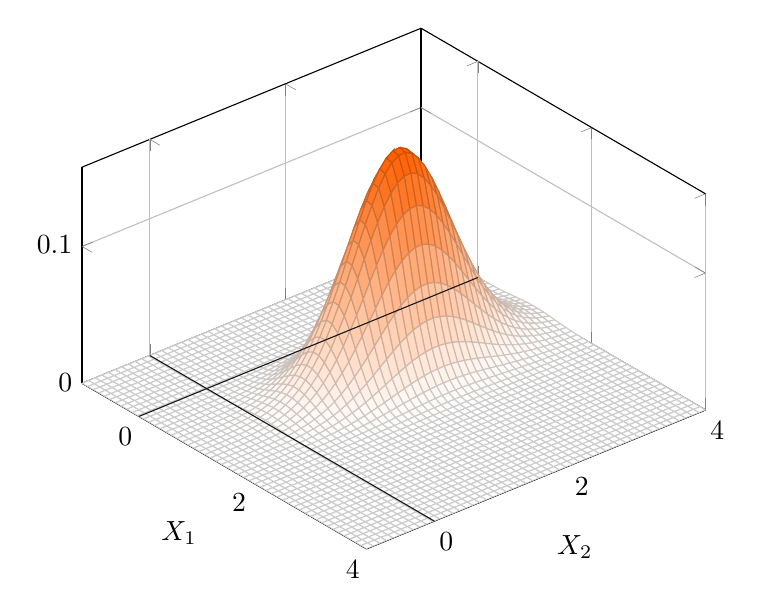
\begin{tikzpicture}[
        declare function={mu1=1;},
        declare function={mu2=2;},
        declare function={sigma1=0.5;},
        declare function={sigma2=1.0;},
        declare function={normal(\m,\s)=1/(2*\s*sqrt(pi))*exp(-(x-\m)^2/(2*\s^2));},
        declare function={bivar(\ma,\sa,\mb,\sb)=
        1/(2*pi*\sa*\sb) * exp(-((x-\ma)^2/\sa^2 + (y-\mb)^2/\sb^2))/2;}]
        \begin{axis}[
          colormap name=whitered,
          width=9.5cm,
          view={50}{45},
          enlargelimits=false,
          grid=major,
          domain=-1:4,
          y domain=-1:4,
          samples=52,
          xlabel=$X_1$,
          ylabel=$X_2$,
          % axis on top, % Ensure grid lines are drawn on top
          ]
          \addplot3 [surf] {bivar(mu1,sigma1,mu2,sigma2)};
          \draw [black!90] (axis cs:-1,0,0) -- (axis cs:4,0,0);
          \draw [black!90] (axis cs:0,-1,0) -- (axis cs:0,4,0);      
        \end{axis}
      \end{tikzpicture}
    \end{column}
    \begin{column}{0.275\textwidth}
      \[ \bm{\mu} = \bmx 1 & 2 \emx \]
      \[ \bm{\Sigma} = \bmx 0.5 & 0 \\ 0 & 1.0 \emx \]
    \end{column}
  \end{columns}
\end{frame}

\end{document}